%******************************************************
%*    LaTex-Vorlage für wissenschaftliche Arbeiten    *
%*    --------------------------------------------    *
%*      Autor: Jan Brennenstuhl (@jbspeakr)           *
%*             www.funkblocka.de                      *
%*            Lizenz: CC BY-SA 3.0                    *
%******************************************************
%*  Anmerkung: Unter Verwendung der Paket-            *
%*             Empfehlungen von Georg Verweyen und    *
%*             Teilen der Vorlage von Tino Weinkauf   *
%******************************************************

% Einstellungen
\pdfminorversion=6
\documentclass[
  oneside,
  paper=A4, 		% Stellt auf A4-Papier ein
  pagesize, 		% Diese Option reicht die Papiergröße an alle Ausgabeformate weiter
  DIV=calc, 		% Für einen guten Satzspiegel
  headings=small,	% Für etwas kleinere Überschriften
  english,  		% Neue Rechtschreibung (Silbentrennung)
  12pt, 			% Schriftgröße
  listof=totoc, 
  bibliography=totoc, 
  index=totoc, 
]{scrbook}
% ---------------------------------------------------------------
% Unverzichtbare Pakte
\usepackage[T1]{fontenc}	% für Texte mit Umlauten und/oder Akzenten 
\usepackage[utf8]{inputenc}	% Silbentrennung und Eingabe von Umlauten
% \usepackage{fixltx2e}  		% Verbessert einige Kernkompetenzen von LaTeX2e
\usepackage{natbib} 
\usepackage{graphicx} 		% Einfügen von Grafiken (.png)

\usepackage[acronym,toc,nonumberlist,nopostdot]{glossaries-extra}
\makenoidxglossaries 
\GlsXtrLoadResources[src={./etc/acronym}]
% \glsaddall
%Change Legends
\usepackage{caption}
\captionsetup{
    labelfont=bf,
    skip=4pt
}
% \usepackage[hyphens]{url} 	% URL's schöner formatieren
% \usepackage[pdftex,a4paper,breaklinks,bookmarksnumbered]{hyperref}  % Hyperlinks im PDF-Dokument
%\usepackage{pdfpages} 		% Einfügen von PDF-Dateien
\usepackage[english]{babel} 	% 
% \begin{otherlanguage}{ngerman}
  % Your German content here
% \end{otherlanguage}
% ---------------------------------------------------------------
% Typografisch empfehlenswerte Pakete
% \usepackage{
%   ellipsis, % Korrigiert den Weißraum um Auslassungspunkte
%   ragged2e, % Ermöglicht Flattersatz mit Silbentrennung
%   marginnote,% Für bessere Randnotizen mit \marginnote statt % \marginline
% }
% \usepackage[tracking=true]{microtype}%
% \DeclareMicrotypeSet*[tracking]{my}% 
%   { font = */*/*/sc/* }% 
% \SetTracking{ encoding = *, shape = sc }{ 45 }% alle Passagen in Kapitälchen automatisch leicht gesperrt.
% ---------------------------------------------------------------

% Set the path for images
\graphicspath{{./images/}}

% Input hyphenation rules
\input{./etc/hyphenation}
% ---------------------------------------------------------------

% Verschiedene Schriften
\usepackage{%
  lmodern, % A) Latin Modern Fonts sind die Nachfolger von Computer
            % Modern, den LaTeX-Standardfonts
%  hfoldsty % B) Diese Schrift stellt alle Ziffern, außer
            % im Mathemodus, auf Minuskel- oder Mediäval-Ziffern um.
            % Wenn Ihre pdfs unscharf aussehen installieren Sie bitte
            % die cm-super-Fonts (Type1-Fonts).
% charter   % C) Diese Zeile lädt die Charter als Schriftart
}
% ---------------------------------------------------------------
% Glossar-Anpassungen
% Den Punkt am Ende jeder Beschreibung deaktivieren
\renewcommand*{\glspostdescription}{}

% ---------------------------------------------------------------

% Hier startet der Inhalt
\begin{document}
% Meta-Informationen für das PDF
\input{./etc/pdf-info}
% Titelblätter und Erklärung
\frontmatter
%******************************************************
%*    LaTex-Vorlage für wissenschaftliche Arbeiten    *
%*    --------------------------------------------    *
%*      Autor: Jan Brennenstuhl (@jbspeakr)           *
%*             www.funkblocka.de                      *
%*            Lizenz: CC BY-SA 3.0                    *
%******************************************************
% Deckblatt
% -----------------------------------------------------
\thispagestyle{empty}
\begin{center}
		
		% Das Logo der Uni (im image-Ordner)
    % 
\includegraphics[width=3cm]{images/Potsdam_logo}\\
    % \vspace{.5cm}

% Logos der Institute nebeneinander
\begin{minipage}[t]{0.45\textwidth}
  \centering
  
\includegraphics[width=3cm]{images/Potsdam_logo}\\
\end{minipage}
\hfill  % Adds horizontal space between the two minipages
\begin{minipage}[t]{0.45\textwidth}
  \centering
  
\includegraphics[width=5cm]{images/logo-ibdm-couleur}\\
\end{minipage}

    
    % % Der Name deiner Uni
    % {\Large Universität Potsdam}\\
    % \vspace{1cm}
    
    % % Der Name deines Instituts
    % {\Huge Institut für Informatik\\[1mm]}
    
    % Der Titel deiner Arbeit (in originaler Sprache)
    \vspace{0.5cm}
    {\Huge \textbf{Mitochondrial Metabolic}}\\
    \vspace*{2mm}
    {\Huge \textbf{Modeling in}}\\
    \vspace*{2mm}
    {\Huge \textbf{Cortical Development}}\\
    \vspace*{3mm}
    % {\Huge \textbf{deiner Arbeit}}\\
    % \vspace*{3mm}
    % {\large \textbf{inklusive Untertitel}}\\
    
    % Eine formelle Einleitung
    \vspace{2.0cm}
    {\large Submitted to the}\\
    {\large Chair of Bioinformatics}\\
    {\large at the}\\
    {\large Institute of Biochemistry and Biology}\\    
    {\large University of Potsdam}\\
    \vspace{0.5cm}
    {\large in partial fulfillment of the requirements for the degree of}\\
    \vspace{1cm}
    
    % Dein zukünftiger akademischer Grad
    {\Large  Master of Science}\\
    \vspace{0.5cm}
    {\large by}\\
    \vspace{2mm}
		% Deine Anrede
    \Large{Maëlle Spiller}\\
    \vspace{1cm}
    %Datum
    {\small May 2026}
    \vspace{1cm}
  \centering
  % Supervisors section
  \begin{large}
    \begin{tabbing}
      1st Supervisor: \= Dr. Bianca Habermann\\
      2nd Supervisor: \> Prof. Zoran Nikoloski
    \end{tabbing}
  \end{large}
  \vspace{1.5mm} 

  \end{center}

\newpage
 


% ---------------------------------------------------------------
% % Glossar
% \include{./etc/glossary}
% ---------------------------------------------------------------
% Quellen
% \bibliography{literature}
% \newcites{literature}{Literaturverzeichnis}

% ---------------------------------------------------------------
---------------------------------------------------------------
% Befehl für Überschriften mit Untertitel
\newcommand{\Chapter}[2]{\chapter[#1]{#1:\\#2}} 
\newcommand{\Section}[2]{\section[#1]{#1:\\#2}}
% ---------------------------------------------------------------
% Danksagung
% \include{./intro/ThankYou}

% Abstract
%******************************************************
%*    LaTex-Vorlage für wissenschaftliche Arbeiten    *
%*    --------------------------------------------    *
%*      Autor: Jan Brennenstuhl (@jbspeakr)           *
%*             www.funkblocka.de                      *
%*            Lizenz: CC BY-SA 3.0                    *
%******************************************************
% Deutsche Zusammenfassung
\begin{center}
    \textbf{Zusammenfassung}
\end{center}
\vspace*{1cm}
% -----------------------------------------------------
Während der Entwicklung des murinen Neokortex am embryonalen Tag \gls{E} 14.5 ist bereits eine kortikale Schichtung etabliert, wobei neuronale Progenitorzellen apikal lokalisiert sind, während neu entstandene Neuronen zur basalen Oberfläche migrieren. 
Diese unterschiedlichen räumlichen Lokalisationen setzen die Zellen vermutlich verschiedenen Umgebungsbedingungen aus, welche den mitochondrialen Stoffwechsel während der embryonalen Neurogenese beeinflussen. Um diese metabolischen Anpassungen 
zu untersuchen, integrierten wir E14.5-Maus-Single-Cell-RNA-Sequenzierungsdaten aus dem Vorderhirn 
in das mitochondriale Genome-Scale-Metabolic-Model MitoMammal \citep{CHAPMANMitoMAMMALGenomeScale2025}, um 
zelltyp-spezifische metabolische Netzwerke zu generieren. 
\newline

Da die Sauerstoffverfügbarkeit den mitochondrialen Stoffwechsel maßgeblich beeinflusst, 
etablierten wir zunächst physiologisch relevante Sauerstoffrestriktionen für jede Zelltypklasse.
Mithilfe eines E-Flux-basierten Ansatzes identifizierten wir Plateaus der Komplex-V-Aktivität der mitochondrialen Atmungskette bei steigender Sauerstoffaufnahme und kombinierten diese Ergebnisse mit Literaturdaten, um zelltypspezifische Sauerstoffrestriktionen zu definieren. Bemerkenswerterweise zeigten Vorgängerpopulationen eine zunehmende Komplex-V-Aktivität mit steigender Sauerstoffverfügbarkeit, was darauf hindeutet, dass diese Zellen metabolisch bereits auf oxidative Phosphorylierung vorbereitet sind.
\newline 

Anschließend verwendeten wir einen gewichteten iMAT-Ansatz, der neben hoch exprimierten Genen auch moderat exprimierte Reaktionen berücksichtigt, um reduzierte, kontextspezifische metabolische Modelle zu erzeugen. Mittels Subsampling-Analysen konnten wir zeigen, dass weighted iMAT robuste Lösungen liefert und die Identifikation robuster Kernreaktionen über verschiedene Zelltypen hinweg ermöglicht. Insgesamt etabliert dieser Ansatz umweltabhängig eingeschränkte metabolische Modelle für die embryonale Neurogenese und schafft eine Grundlage zur Untersuchung metabolischer Anpassungen während der kortikalen Entwicklung. 

% -----------------------------------------------------
% Englische Zusammenfassung
\newpage
\vspace*{1cm}
\begin{center}
    \textbf{Abstract}
\end{center}
\vspace*{1cm}
% -----------------------------------------------------
During mouse neocortical development at embryonic day (E) 14.5, cortical layering is already established, with neural progenitor cells localized apically while newly generated neurons migrate toward the basal surface. These distinct spatial localizations likely expose cells to different microenvironmental conditions that influence mitochondrial metabolism during embryonic neurogenesis. To investigate these metabolic adaptations, we integrated E14.5 mouse single-cell RNA sequencing data from the forebrain into the MitoMammal \citep{CHAPMANMitoMAMMALGenomeScale2025} mitochondrial genome-scale metabolic model to generate cell type–specific metabolic networks.
\newline

Because oxygen availability strongly influences mitochondrial metabolism, we first established physiologically relevant oxygen constraints for each cell type class. Using an E-Flux–based approach, we identified mitochondrial Complex V activity plateaus across increasing oxygen uptake levels and combined these results with literature-derived information to define cell type–specific oxygen constraints. Notably, progenitor populations displayed increasing Complex V activity with oxygen availability, suggesting that these cells are metabolically prepared for oxidative phosphorylation. 
\newline

We then applied a weighted iMAT framework, which in addition to highly expressed genes also rewards moderately expressed reactions, to derive reduced context-specific metabolic models. Through subsampling analyses, we demonstrated that weighted iMAT generates robust solutions and enables the identification of robust core reactions across cell types. Altogether, this framework establishes environmentally constrained metabolic models for embryonic neurogenesis and provides a basis for studying metabolic adaptations during cortical development. 


% Inhaltsverzeichnis
\tableofcontents 
% ---------------------------------------------------------------
% Hauptteil - Arabische Seitennummerierung
\mainmatter % die eigentliche Arbeit
\pagenumbering{arabic}
% Akronyme
% \newacronym{PKI}{PKI}{Public-Key Infrastructure}
\newacronym{IDM}{IDM}{Identity Management}
\newacronym{ESB}{ESB}{Enterprise Service Bus}
\newacronym{ID}{ID}{Identifier}
\newacronym{SigG}{SigG}{Signaturgesetz}
\newacronym{CCC}{CCC}{Chaos Computer Club e. V.}
\newacronym{BSI}{BSI}{Bundesamt für Sicherheit in der Informationstechnik}
\printnoidxglossary[type=\acronymtype, title=List of Acronyms]


%******************************************************
%*    LaTex-Vorlage für wissenschaftliche Arbeiten    *
%*    --------------------------------------------    *
%*      Autor: Jan Brennenstuhl (@jbspeakr)           *
%*             www.funkblocka.de                      *
%*            Lizenz: CC BY-SA 3.0                    *
%******************************************************
\chapter{Biological Introduction}
\label{chap:bioIntr}
\section{From a Neural Tube to the Central Nervous System}
The whole central nervous system \gls{CNS}, including the brain, brainstem and the spinal cord, 
emerges from a single layered neural tube that is formed early in vertebrate development through the process of 
neurulation. By the time it closes (around embryonic day \gls{E} 9.5-10.5 in mice and E25-27 in humans), 
the neural tube already exhibits distinct anteroposterior and dorsoventral patterning, giving rise to the three primary brain vesicles: the forebrain 
(Prosencephalon), midbrain (Mesencephalon), and hindbrain (Rhombencephalon) \citep{SAKAINeurulationMouseManner1989}. The forebrain is further divided into the Diencephalon and the telencephalon, which, once fully developed, comprises the cerebral cortex, including hippocampus and neocortex, as well as the basal ganglia and olfactory bulb.

%IMAGE BRAIN VESSEL
\begin{figure}[h]
    \centering
    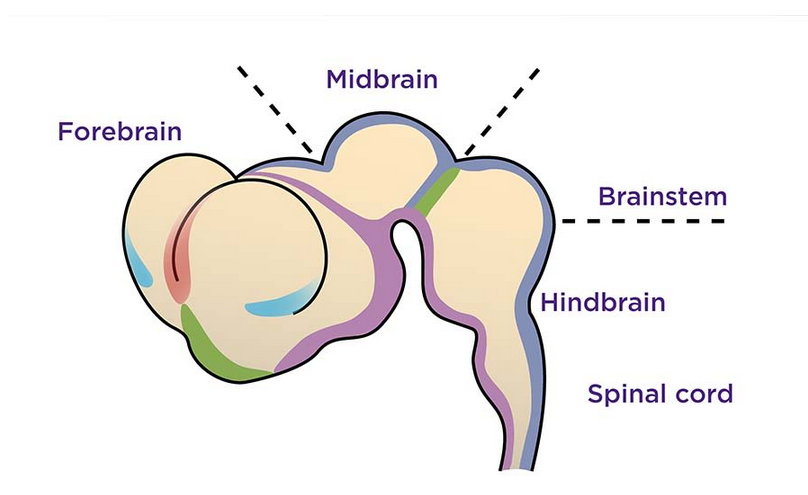
\includegraphics[width=0.7\textwidth]{brain_vessels.png}
    \caption{\textbf{Formation of the three primary brain vesicles during early neural development.} The neural tube is already regionalized into distinct structures corresponding to the forebrain, midbrain, and hindbrain. \textcopyright Queensland Brain Institute, University of Queensland, Australia. }
    \label{fig:brainVessel}
\end{figure}
% -----------------------------------------------------
\section{Neurogenesis generates Neural Diversity}
With the closure of the neural tube, a series of tightly regulated processes initiate the formation of the complex brain. At this stage, the neural tube consists of just a single layer of neuroepithelial stem cells \glspl{NSC},
which must first undergo population expansion to generate sufficient progenitors for subsequent developmental stages. Between E8 and E10, 
NSCs undergo rapid symmetric division, a phase referred to as the expansion phase. Once an adequate number of NSCs has been established, neurogenesis begins. 


Neurogenesis refers to the formation of neurons from NSCs and its neural progenitor cells \glspl{NPC} \citep{SUNGrowthFoldingMammalian2014}, and occurs throughout the whole neural tube. In rodents, neurogenesis spans approximately E10.5 to E18.5 \citep{GOTZCellBiologyNeurogenesis2005}, followed by radial neuronal migration, differentiation, as well as the formation of dendrites and axons for interconnection within the neural network \citep{KRIEGSTEINPatternsNeuronalMigration2004}.


Neurogenesis is initiated by a switch from symmetric to asymmetric division of NECs. During these self-renewing asymmetric divisions, one daughter cell retains NEC identity, while the other differentiates into an apical radial glial cell, which we will refer to as apical progenitor \gls{AP} \citep{GOTZCellBiologyNeurogenesis2005}.

%IMAGE Neurogenesis
\begin{figure}[h]
    \centering
    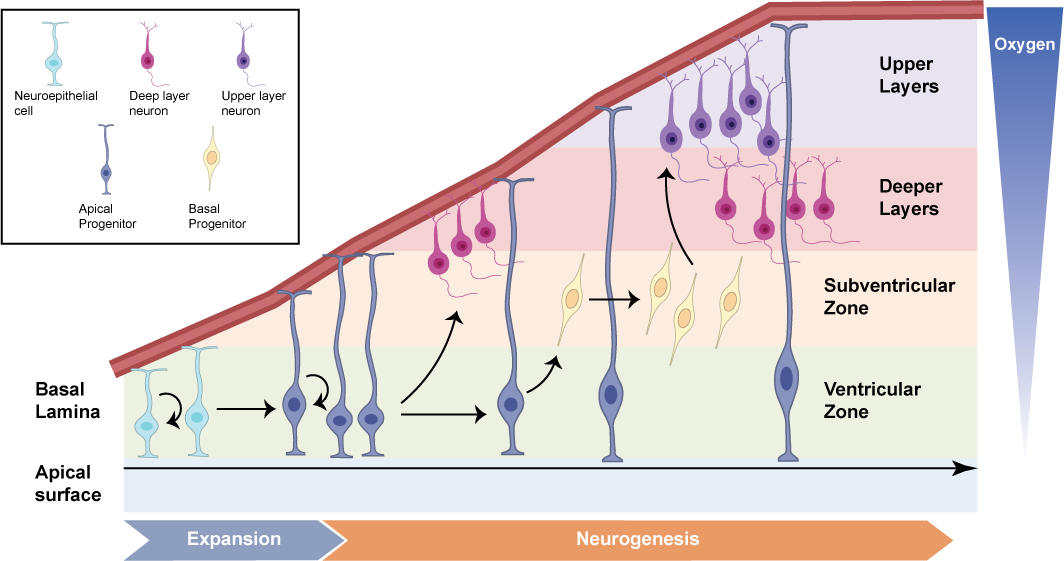
\includegraphics[width=0.7\textwidth]{neurogenesis.png}
    \caption{\textbf{Development of the mouse neocortex.} Schematic overview of neocortical development in the mouse. During early embryogenesis (E9.5–E11.5), neuroepithelial cells (NECs) in the ventricular zone \gls{VZ} undergo symmetric proliferative divisions, expanding the progenitor pool. Around E11.5, NECs transition into apical progenitors (APs), which initially self-renew and subsequently enter a neurogenic phase. Between E11.5 and E13.5, APs generate early-born deep-layer neurons (DLNs), which migrate basally toward the cortical plate. From approximately E13.5 onward, APs also produce basal progenitors (BPs) that populate the subventricular zone (SVZ) and give rise to late-born upper-layer neurons (ULNs). Blood vessels invade radially from the basal lamina toward the apical surface, suggesting the establishment of an oxygen gradient decreasing from basal to apical regions. Figure created with BioRender.com.
    }
    \label{fig:neurogenesis}
\end{figure}


% -----------------------------------------------------
\section{Apical Progenitors}
Both, NECs and APs reside within and divide in the same germinal zone, the ventricular zone \gls{VZ}, which is defined by its direct contact with ventricles that are cerebrospinal fluid filled on the apical side. APs exhibit several characteristic features: (1) an elongated 
morphology with both apical and basal processes, allowing direct contact with the ventricular and pial surfaces. (2) interkinetic nuclear migration (INM), a process in which the nucleus moves from the apical toward the basal side during the cell cycle, while mitosis occurs at the ventricular surface and (3) the expression of astroglial marker genes such as nuclear Pax6 (Paired box 6), Sox2 (sex determining region Y-box 2) \citep{GOTZPax6ControlsRadial1998}, glutamate transporter (GLAST) (Shibata et al. 1997), glial fibrillary acidic protein (GFAP)
\citep{LEVITTImmunoperoxidaseLocalizationGlial1980}, and  glutamine synthetase \gls{GS} \citep{ENGLUNDPax6Tbr2Tbr12005}.


APs represent a distinct and versatile progenitor population, capable of adopting multiple cell fates during neocortex development. Following an initial expansion phase (~ E10-E12) , APs undergo a progressive shift toward asymmetric cell division. In the first phase of asymmetry divisions (~E12-E13), APs generate postmitotic neurons destined for deep cortical layers (deep-layer neuron, \gls{DLN}). 


As neurogenesis proceeds (~E13-E16), their asymmetric division increasingly gives rise to more differentiated progenitor populations: basal progenitors \glspl{BP}.
In comparison to NECs and APs, BPs detach from the apical surface and migrate outward to establish the secondary germinal layer, called the subventricular zone \gls{SVZ}.


% -----------------------------------------------------
\section{Basal Progenitors}

Basal progenitors represent a heterogeneous secondary progenitor class that are more difficult to clearly separate from other cell types. While some BPs fully detach from the ventricular surface, others retain a basal process and maintain a gene expression profile more closely related to their AP origin \citep{pilzAmplificationProgenitorsMammalian2013}. 
Basal radial glia, for example, represents a minority of BPs in rodents, accounting for approximately 5\% \citep{MARTINEZ-CERDENOComparativeAnalysisSubventricular2012}, and are still attached to the basal surface. 


Basal intermediate progenitors on the other hand, represent a major subclass in BPs and are no longer in contact with either the apical or basal surface. Furthermore, basal intermediate progenitors exhibit limited proliferative capacity in comparison to APs. They typically undergo a single proliferative division, before producing two upper layer neurons \glspl{ULN} \citep{THORIndirectNeurogenesisSpace2024}. 
In addition, they are characterized by different marker gene expression, including Tbr2/Eomes (T-box brain protein 2/Eomesodermin) \citep{ENGLUNDPax6Tbr2Tbr12005}. Here, BPs refers specifically to the subclass of basal intermediate progenitors. 

% -----------------------------------------------------
\section{Migration Of Upper-Layer And Deep-Layer Neurons}

DLNs and ULNs originate from distinct progenitor populations within the developing neocortex. DLNs are primarily generated by APs in the VZ, while ULNs arise from BPs in the SVZ. Regardless of their origin, both neuronal populations must undergo radial migration towards the pial surface in order to reach their final positions in the deeper and upper layers of the neocortex, respectively \citep{NADARAJAHModesNeuronalMigration2002}.


Two principal modes of radial migration have been described. In early stages, neurons predominantly undergo somal translocation, a process in which the neurons extend a basal process that anchors to the pial surface while the nucleus moves along this process toward the basal side, resulting in progressive shortening of the process while maintaining attachment. At later stages, neurons primarily adopt a locomotion-based mode of migration, also referred to as gliophilic migration, in which they migrate along radial glial fibers of APs \citep{NADARAJAHModesNeuronalMigration2002}.
Through radial migration along the fibers of APs, DLNs settle near the pial surface and form the initial cortical layer. As neurogenesis progresses, ULNs migrate past these earlier-born cells to establish progressively more superficial layers \citep{BUCHSBAUMNeuronalMigrationCNS2019}.


This sequential pattern of migration and positioning results in the characteristic inside-out organization of the cortex, whereby early-born neurons occupy deeper layers and later-born neurons populate the upper layers.
% -----------------------------------------------------

\section{Vascularization and Oxygen Dynamics in the Developing Cortex
}
In addition to the generation of new cells in the neocortex, the developing brain must also establish a reliable supply of nutrients and oxygen. Vascularization begins in mice around E8.5–E10 with the formation of a vascular network surrounding the neural tube, called the perineural vascular plexus \citep{HOGANNeuralTubePatterns2004},
reviewed in \citep{JAMESNeuronalActionDeveloping2011}. From this outer network, new blood vessels grow radially from the pial toward the ventricular (apical) zone. Before reaching the inner (apical) surface of the neural tube, these vessels turn and extend sideways, where they connect with one another to form an internal vascular network, referred to as the subventricular vascular plexus \citep{TATAVascularisationCentralNervous2015, FANTINNRP1ActsCell2013}.


Importantly, this process is not uniform across the CNS. While the hindbrain and spinal cord are vascularized relatively homogeneously, the forebrain exhibits a temporal delay, with blood vessels initially invading ventral regions while dorsal areas remain temporarily avascular \citep{VASUDEVANCompartmentspecificTranscriptionFactors2008}.

Oxygen levels have been shown to play a critical role during neocortex development. Hypoxia during fetal development can disrupt cortical progenitor cell growth, leading to brain abnormalities such as smaller overall brain size, thinner cortex or enlarged ventricles \citep{piesovaImpactPerinatalHypoxia2020}.
In most studies, oxygen levels are quantified using  arterial partial oxygen tension PO$_2$, where atmospheric oxygen levels correspond to a PO$_2$ of 21\% (150mmHg).


Even though hypoxia can disrupt normal brain development under pathological conditions, physiological hypoxia is essential in maintaining normal developmental processes. For instance, the stemness of NSCs is preserved under physiological hypoxic conditions \citep{EZASHILowO2Tensions2005}, aligning with observations that oxygen levels in the forebrain are significantly lower (PO$_2$ = 1-6\%) during development \citep{LEEDeterminationHypoxicRegion2001,ZHANGOxygenKeyFactor2011}. Within this hypoxic environment, the SVZ reaches slightly higher PO$_2$ values (2.5-3\%) \citep{SANTILLIMildHypoxiaEnhances2010}.


Similarly, the differentiation of NPCs into neurons is regulated by local oxygen levels \citep{malikNeurogenesisContinuesThird2013},  and increased oxygen availability has been associated with enhanced neuronal differentiation \citep{STORCHFunctionalCharacterizationDopaminergic2003,SASANTILLIMildHypoxiaEnhances2010,STUDEREnhancedProliferationSurvival2000}.


Consistent with these findings, NSC differentiation has been shown to coincide with blood vessel ingrowth \textit{in vivo} \citep{SHENEndothelialCellsStimulate2004}, that is accompanied by increased tissue oxygenation and reduced levels of HIF-1\textalpha, 
a key hypoxia marker. Additionally, evidence from genetic knockout supports a causal role of oxygen in cortical development. In Gpr124 knockout embryos, which exhibit impaired brain vascularization, oxygen levels fail to increase within the stem cell niche, resulting in sustained AP expansion at the expense of differentiation. Notably, experimentally increasing tissue oxygenation does not rescue vascular defects but is sufficient to reduce HIF-1\textalpha 
levels and restore progenitor differentiation \citep{LANGEReliefHypoxiaAngiogenesis2016}.

While the temporal dynamics of vascularization during cortical development are relatively well understood, far less is known about the spatial distribution of oxygen within the developing cortex. Studies in the adult brain have revealed the presence of gradients, where oxygen levels decline along the length of capillaries due to consumption by surrounding cells. These gradients are particularly pronounced in grey matter, which is densely populated with neurons and exhibits a steeper oxygen drop-off compared to white matter, where myelinated axons reside. Notably, while grey matter shows sharper gradients, absolute PO$_2$ 
values tend to be lower in white matter \citep{erecinskaTissueOxygenTension2001}.

In addition to the extracellular oxygen gradients, intracellular oxygen gradients are also assumed to exist in the brain, particularly in neurons, which maintain high rates of oxygen consumption. Within these cells, mitochondria may create localized regions of lower oxygen tension due to rapid oxygen utilization.

Given that blood vessels invade the cortex radially from the pial surface toward deeper regions, it is reasonable to infer the existence of a spatial oxygen gradient. In such a scenario, more superficial regions populated by ULN and DLN would experience higher oxygen availability, whereas deeper regions including the VZ and SVZ that harbor neural stem and progenitor cells, would remain comparatively hypoxic. 

-----------------------------------------------------
\section{From Embryonic Neurogenesis to Postnatal and Adult Neurogenic Processes}
Toward the end of neurogenesis (~E16.5 onward), progenitor cells transition from neurogenesis to gliogenesis, giving rise to distinct glial precursors that subsequently differentiate into astrocytes and oligodendrocytes \citep{VIEIRANeuralStemCell2018}.
In the present work, however, we focus exclusively on neurogenic processes and do not further address gliogenesis.
% -----------------------------------------------------

\section{Species-Specific Differences: From Rodent Models to Human Brain Development}
With respect to rodents such as mice and rats, which are widely used as laboratory models, it is important to note that most mammals possess larger and more complex brains. This increased complexity is reflected in greater cellular diversity, additional cortical layers, and fundamental differences in developmental dynamics. For instance, neurogenesis in the human cortex is markedly prolonged, lasting approximately 141 days compared to around 11 days in mice, and is accompanied by an extended proliferative phase and longer cell cycle durations in human NPCs \citep{LIBE-PHILIPPOTCellularMolecularMechanisms2021}.

Structural differences further highlight this divergence. The proliferative SVZ is substantially expanded in humans and subdivided into an inner and outer SVZ. Within the outer SVZ, BPs are greatly enriched and have been closely associated with increased brain size and cortical expansion \citep{reilloRoleIntermediateRadial2011}. In addition, BPs in humans exhibit enhanced proliferative capacity compared to their rodent counterparts. Finally, these developmental and cellular differences are paralleled by large-scale anatomical distinctions, as mice are lissencephalic, possessing smooth brains, whereas humans exhibit gyrencephaly, characterized by varying degrees of cortical folding \citep{BORRELLHowCellsFold2018}.

Nevertheless, the cerebral cortex of rodents and humans share fundamental structural and functional properties, including layered organization, and similar developmental sequences \citep{luhmannCanWeUnderstand2020},  that allows detailed \textit{in vivo} and \textit{in vitro} analyses, as well as 
specific experimental manipulations.

% -----------------------------------------------------

\section{Developmental Dynamics during Neurogenesis}
Development is not a static process, but a finely tuned interplay of coordinated dynamics, that guide cell behavior at every step. By dynamics, we mean the continuous changes in a cell’s internal state, including its transcriptome, proteome, and metabolome, as well as the evolving external milieu of signaling molecules, mechanical forces and environmental cues.

Together, these dynamics shape the structure of the cortex. They drive the transition of NSCs and NPCs from multipotency to lineage-restricted states, ultimately giving rise to specialized neural and glial identities. Additionally, they regulate the balance between self-renewal and differentiative state.

% -----------------------------------------------------
\section{Transcriptomical Dynamics}
Advances in high-resolution molecular profiling have begun to transform our understanding of these developmental processes by enabling the characterization of cellular states at a remarkably detailed view (reviewed in \citep{BRISCOELookingNeurodevelopmentBig2020}).  In particular, single-cell RNA sequencing 
\gls{scRNA-seq} and spatial transcriptomic approaches have substantially refined our understanding of individual cell types and developmental trajectories throughout cortical development. For example, these technologies have revealed that NPCs and their progeny transition through a series of transient molecular states, characterized by sequential activation and repression of gene networks. This dynamic transition of transcriptional profiles not only distinguishes emerging cell types, but also occurs within individual progenitor populations 
\citep{RUANProgenitorCellDiversity2021}, where cells exhibit asynchronous progression and diverse lineage trajectories. 

% -----------------------------------------------------
\section{Temporal Remodeling of the Transcriptome}
The identity of each cell type is defined by characteristic marker gene expression patterns, yet during neurogenesis the transcriptome undergoes extensive and continuous remodeling, which complicates the characterization of cell types during embryonic development. Early embryonic mouse brain studies have demonstrated that as much as 10–13 \% of mRNAs and proteins change in expression within a two-day developmental window \citep{HARTLTranscriptomeProteomeAnalysis2008}. 
At E9.5, gene expression is dominated by transcripts associated with metabolism and the cell cycle, reflecting active proliferation. By E11.5 and E13.5, coinciding with the transition from progenitor states to neuronal differentiation, there is a marked shift toward the expression of genes involved in neuronal identity and function.

Consistent with this view, scRNA-seq analyses of human fetal brain tissue have revealed that neural progenitor populations are not only heterogeneous but also dynamically diverge along distinct developmental trajectories \citep{SILVESTRISSinglecellTranscriptomicProfiling}.
For example, BPs from the SVZ segregate into subpopulations that follow two principal transcriptional programs, leading either toward glial lineages or toward neuronal identities. Similar observations from in vitro systems further support the idea that multiple progenitor subpopulations can coexist while undergoing progressive transcriptional shifts.

Importantly, transcriptional dynamics are not restricted to embryonic development but persist across the lifespan. Spatial and temporal transcriptomic studies in the mouse brain have shown that gene expression profiles continue to evolve from early postnatal stages into adulthood and aging. Early postnatal brains are enriched for transcriptional programs associated with neurogenesis, gliogenesis, and myelination, whereas aged brains exhibit increased expression of genes linked to stress responses and inflammation \citep{CONACHERSpatialTranscriptomicsReveals2025}.
% -----------------------------------------------------
\endinput
\input{./sections/2-Second}
\input{./sections/3-Third}
\input{./sections/4-Fourth}
\input{./sections/5-Fifth}
\input{./sections/6-Sixth}
\input{./sections/7-Seventh}
% ---------------------------------------------------------------
% % Schlussteil - Römische Seitennummerierung
% \backmatter
% \pagenumbering{arabic}
% \setcounter{page}{11}
% ---------------------------------------------------------------
% Quellenverzeichnisse
\bibliographystyle{plainnat}
\typeout{}
\bibliography{literature}

% ---------------------------------------------------------------
% %Glossar ausgeben
% \printglossary[style=altlist,title=Glossar]

% %Abkürzungen ausgeben
% \deftranslation[to=German]{Acronyms}{Abkürzungsverzeichnis}
% \printglossary[type=\acronymtype,style=long]
% ---------------------------------------------------------------
% Anhang
\appendix
%\includepdf[pages=-,fitpaper=true,addtotoc={1,section,0,Diagramm: Vergabe,fig:Vergabedia}]{Pfad-zu-einem-pdf-dokument.pdf}
% ---------------------------------------------------------------

% Erklärung (Arbeit selbstständig verfasst)
\newpage
%******************************************************
%*    LaTex-Vorlage für wissenschaftliche Arbeiten    *
%*    --------------------------------------------    *
%*      Autor: Jan Brennenstuhl (@jbspeakr)           *
%*             www.funkblocka.de                      *
%*            Lizenz: CC BY-SA 3.0                    *
%******************************************************
\begin{large}

\vspace*{2cm}
\noindent
Hereby, I declare that I have composed the present thesis independently on my own and without other sources than the ones indicated. 
All thoughts taken directly or indirectly from external sources are properly denoted as such.
\noindent

\vspace{3cm}
Marseille, 1st of May 2026
\vspace{1cm}

\hspace*{6cm}%
\dotfill\\
\hspace*{7cm}%
\textit{(Signature)}

\end{large}
  

\end{document}
